% -*- TeX-master: "226notes.tex" -*-
\chapter{10.7 (Part One): Power Series: }
\section{Reminders}
\subsection{MATH\_226 Reminders}
\begin{enumerate}
  \item \textbf{MyLab Math 10: Radius and Interval
        of Convergence} is due on \textbf{Friday, April 21,
        2023}.
  \item \textbf{Written Homework 4} is going
        to be due on \textbf{Monday, April 24, 2023}.
\end{enumerate}
\subsection{MATH\_230 Reminders}
\begin{enumerate}
  \item \textbf{MyLab Math 8: Polar Coordinates } is due
        on \textbf{Thursday, April 20, 2023}.
  \item \textbf{MyLab Math 9: Curves in Space and
        Their Tangents} is due on \textbf{Sunday, April
        23, 2023}.
  \item \textbf{MATH\_230-1 Midterm 1} is \textbf{6 days away}. The test will be on \textbf{Tuesday,
        April 25, 2023}.
\end{enumerate}


\section{Objectives}
\begin{enumerate}
  \item Be able to identify and evaluate the coefficients
        of a power series as well as the center of
        the power series.
  \item Represent certian elementary functions as power
        series.
  \item Detemrine whether a power series
        converges at a point by applying convergence
        tests for infinite series
\end{enumerate}

\section{Motivation}
In the past few chapters, we have learned about
sequence and series convergence as well as
their technical intricacies. We have been able to utilize
our knowledge of sequences, series, and limits in order
to develop a baseline understanding of how series and
sequences worked, but we have hardly worked on the
\textbf{applications of series}. Surprisingly, series
show up everywhere, and most importantly, we can
actually create generalizatoins about different series
as well as their behaviors in order to apply them.
The most notable way is applying the idea of series to
polynomials, especially whenever we have series that
after all, just look like \textbf{infinite polynomials}.
I mean, examples that come to mind after all,
are the geometric sequence, the alternating series, etc,
which all have the common form of
\[ \sum_{n=0}^{\infty} a_{n} \cdot r^{n} \]
\[ \Rightarrow a_{0} + a_{1} \cdot r^{1} +
  a_{2} \cdot r^{2} + a_{3} \cdot r^{3} + \cdots \]

The questions that we are trying to pose with power series
are as follows:
\begin{itemize}
  \item If a series looks like a polynomial, does it
        \textbf{behave} like a polynomial?
  \item If a series behaves like a polynomial, how
        can we apply our knowledge of algebraic manipulations
        of polynomials to series?
  \item What do these algebraic manipulations on
        power series suggest about the series itself?
        For example, how does adding one power series
        to another power series affect its
        convergence?
  \item How can we apply calculus to series?

\end{itemize}
\section{Introduction to Power Series and Power Series Convergence}%
\label{sec:label}
In the former section, we discussed the idea of the
power series and how exactly we arrived at its conception.
\begin{itemize}
  \item Recall that a power series is meant to be a
        \textbf{infinite series} that resembles
        an \textbf{infinitely-spanning polynomial}.
        \begin{itemize}
          \item Recall that a polynomial is just any
                expression that utilizes terms of
                varying powers and degrees, such as the
                famous equation of the parabola:
                \[ ax^{2} + bx + c \]
        \end{itemize}
  \item In the most primitive context, we can think
        of a polynomial as an expression of terms
        such that there is some constant $ c $
        multiplied by some expression of $ x $ and $ y $.
        \begin{itemize}
          \item Think of the conic sections for example:
                \[ a(x-h)^{2} + b(y-k)^{2} = c^{2} \]
                We can see that the polynomial here
                is blatantly just a \textbf{constant
                multiplied by some expression of a variable}.
        \end{itemize}

\end{itemize}
Applying this to the idea of a series, let's think
of a series that generates an \textbf{infinite polynomial}
as a series in which we have some constant $ c $
multiplied by some expression of $ x $ that has a
varying power of $ n $.
\begin{itemize}
  \item We will call the expression of $ x $ as
        the \textbf{center} of the power series.
        That is, much like how the expressions
        $ (x-h)$ and $ (y-k)$ denote the
        center of a circle, $ (x-a)$ denotes
        the \textbf{center of convergence} of
        powre series.
\end{itemize}

\begin{center}
  \fbox{
    \parbox{\textwidth} {
      \begin{definition}
        Power Series
      \end{definition}
      A \textbf{power series that is \textit{centered} about
        $ x = 0 $} is a series of the form
      \[ \sum_{n=0}^{\infty} c_{n} x^{n} =
        c_{0} + c_{1}x + c_{2}x^{2} + \cdots + c_{n}x^{n} + \cdots \]
      such that $ c_{n} $ is just a constant term.
      \\ \\
      A \textbf{power series about $ x = a $ } is a
      series of the form
      \[ \sum_{n=0}^{\infty} c_{n}(x-a)^{n} =
        c_{0} + c_{1}(x-a) + c_{2}(x-a)^{2}
        + \cdots + c_{n}(x-a)^{n} + \cdots
      \]
      such that $ c_{n} $ is a constant and
      $ a $ is a constant. \\

    }
  }
\end{center}
Now, if we were to just \textbf{evaluate} this
power series, letting $ c_{n} = 1 $ and letting
$ a = 0 $, then we would obtain the following series.
\begin{remark*}[]
  Relating the Power Series Centered at 0 to the
  Geometric Series
\end{remark*}

\[ \textrm{let $ c_{n} = 1 $ and let $ a = 0 $}\]
\[ \sum_{n=0}^{\infty} c_{n}(x-a)^{n}\]
\[ \Rightarrow  \sum_{n=0}^{\infty} x^{n}\]
Now if we expand this power series out\dots
\[ \Rightarrow \sum_{n=0}^{\infty} x^{n} = x^{0} + x^{1} +
  x^{2} + \cdots + x^{n} \]
\[ \Rightarrow 1 + x + x^{2} + \cdots + x^{n } \]
which looks \textbf{oddly} similar to the
\textbf{geometric series} that we have introduced
at the introduction of series\dots mainly becuase
it is the same geometric series! The idea that the
power series resembles the geometric series is a
very importnat idea in the world of the power series,
as it is important ot understand the idea of the ratio
as well as \textbf{recognizing the patterns between the
  terms of an infinite polynomial}.
\par Recall that we know that the sum of an infinite
geometric series is as follows
\[ \sum_{n=0}^{\infty} a_{n} \cdot r^{n} = \frac{1}{1-r} \]
Although it seems weird, we must be able
to asser that, since the power series
$ \sum_{n=0}^{\infty} x^{n}$ behaves exactly
like the geometric series $ \sum_{n=0}^{\infty} a_{n} \cdot r^{n}$
such that $ r = x $, that they \textbf{must converge
  at the same place}.
\par Therefore, we know that the power series we
have created must converge (or must have a total sum
of)
\[ \sum_{n=0}^{\infty} x^{n} = \frac{1}{1-x} ~ \forall ~
-1 < x < 1 \]
According to what we know about the \textbf{geometric
  series}, then we know that the ratio $ r = x $ must
be less than 1, or at least, must have a value that is less
than 1, such as to ensure that the parital sums
of the series are constantly decreasing, as opposed to just
increasing infinitely.
Therefore, we know that the absolute value of $ x $ or
$ |x| < 1 $.
\subsection{Where Things Change\dots (Series aren't \textit{actually} series\dots)}
\par But don't get things crossed, although we
are currently living in series-land, we must
understand that \textbf{power series and eventually
  Taylor Series are not about the series themselves.}
After all, we aren't actually able to write all of the
partial sums of a series to infinity\dots we are just
really good at understanding their behavior thanks to
our immense knowledge of convergence therems and tests.
That being said, though, in reality, we must really think
of the power series, and any series here going forward,
as \textbf{approximations} of the point of convergence,
or the sum. We can think of any expression of partial
sums as an approximation$ P_{n}(x) $ of the true
sum or point of convergence of the series.


\begin{center}
  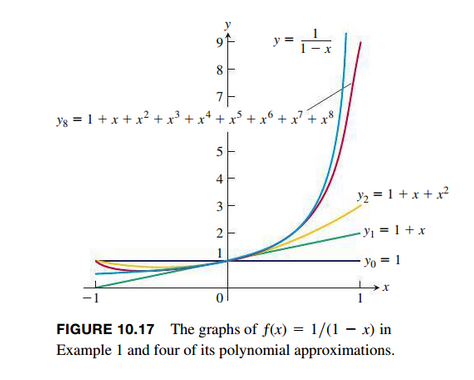
\includegraphics[width = .85\textwidth]{./img/pseriesapprox.png}
\end{center}

Within our image, we can see that the approxmation $ P_{n} ( x )$
improves with the addition of more terms. In the most simple
sense, we are essentially just making the polynomial
derived from the sequence more and more similar to the
graph of the actual function. In this sense, if we were
able to hypothetically add an \textbf{infinite} amount of
terms to the power series, then we would be able to get
an approxmation that is equal to the original function at
some value $ x $.
\begin{remark*}[(2)]
  Find the components of the following series. Then, evaluate
  for what function the series converges to, what the
  radius of convergence is, as well as the infinite sum
  that represents the series.
  \[ 1 - \frac{1}{2}(x-2) + \frac{1}{4} (x-2)^{2} + \cdots
  + \Biggr( -\frac{1}{2}\Biggr)^{n} (x-2)^{n} \]
\end{remark*}

Recall that whenever we are dealing with a power series,
we are trying to think of the terms of the series as
terms within a \textbf{polynomial}. The general form of a
power series is as follows:

\[ \sum_{n=0}^{\infty} c_{n}(x-a)^{n} \]
\[\Rightarrow c_{0} + c_{1}(x-a) + c_{2}(x-a)^{2} +
  c_{3}(x-a)^{3} + \cdots c_{n}(x-a)^{n}\]
Whenever we apply this general structure to the
given power series, we can see that the center $ a $ of the
power series must be 2. Additionally, we can see that
$ c_{0} = 1 $, $c_{1} = - \frac{1}{2}$, $c_{2} = \frac{1}{4}$,
and $ c_{n} = \Biggr( - \frac{1}{2}\Biggr)^{n}$.
Therefore, we are able to translate this power series
to the following infinite sum.

\[ \Rightarrow \sum_{n=0}^{\infty} \Biggr( - \frac{1}{2}  \Biggr)^{n} (x-2)^{n} \]

Because both of the terms of hte power series are
functions of $ n $, then we are able to rewrite the series
in terms of one single ratio $ r$:
\[ \Rightarrow \sum_{n=0}^{\infty} \Biggr( - \frac{(x-2)}{2}  \Biggr)^{n }\]

Given that the infinite sum has the form of a
\textbf{geometric series}, we are able to determien its
\textbf{radius of convergence} knowing that the $ |r| < 1 $.
\[ \Biggr| - \frac{x-2}{2}  \Biggr| < 1 \]
\[ \Rightarrow \Biggr| \frac{x-2}{2}  \Biggr| < 1 \]
\[ \Rightarrow 0 < x < 4 \]
We know that the series will converge only for values of
$ x \in (0,4)$. In order to determine what the series
actually converges to, we are able to apply the
\textbf{sum of a geometric series formula}.
\[ \frac{1}{1-r}\]
\[ \Rightarrow \frac{1}{1+\frac{x-2}{2}}\]
\[ \Rightarrow \frac{2}{2 + x - 2 }\]
\[ \Rightarrow \frac{2}{x}\]
We know that our infinite sum is meant to represent the
function $ f(x) = \frac{2}{x}$ for all values $ x \in (0, 4)$.
The polynomial $ P(n) $, which is equal to the series that
we are given, gives aproximations to the function $ f(x) = \frac{2}{x}$ for any value of $ x $ near 2. From this, we
are able to determine that the following partial sums
\[ P_{0}(x) = 1\]
\[ \Rightarrow  P_{1}(x) = 1 - \frac{1}{2}(x-2)\]
\[ \Rightarrow P_{2}(x) = 1 - \frac{1}{2}(x-2) +
  \frac{1}{4}(x-2)^{2} \]

are just approximations of the function $ \frac{2}{x}$  that
get more and more accurate with the addition of more terms.

Note, though, power series are not just restricted to
geometric series, as we can derive power series (and
approximations of functions with polynomials) with
other types of series.

\section{The Convergence Theorem of Power Series}
Our experiemntation with power series convergence
leads us to the following theorem: \textbf{the Convergence
  Theorem of Power Series}, which offers us a general
idea of how convergence works for power series-- that is,
how we can determine what values of $ x $ the power
series converges to.
\begin{center}
  \fbox{
    \parbox{\textwidth} {
      \begin{thm}
        Convergence Theorem of Power Series
      \end{thm}
      If the power series
      \[ \sum_{n=0}^\infty a_{n}x^{n} =
        a_{0} + a_{1}x + a_{2}x^{2} + a_{3}x^{3} +
        \cdots \]
      converges at $ x = c \neq 0 $, then it
      converges absolutely $ \forall $ such that
      $ |x| < |c| $. If the series diveresg at $ x = d $,
      then it diverges $ \forall $ x such that
      $ | x | > | d | $.
          }
  }
\end{center}
Essentially, this theorem tells us that if we have a
power series that is centered at $ x = 0 $, then if the
series converges at some nonzero value $ c $, then $ x $
will converge for all values within the interval $ - c < x
< c $ and if we know that a power series diverges at $ x = d $,
then the series will diverge for all values of $ x < d $ and
$ x > d $.
\par Note that the theorem does \textit{not} tell us
whether or not that if $ x = c $, then $ c $ is the
\textit{endpoint} of convergence. It merely states that any value
below $ c $ will converge.
\par The other issue with this theorem, though, is that
although it does give us a general idea of the behavior
of a convergent power series, it only offers us informatoin
on the behavior of a convergent power series that is
\textit{centered at $ a = 0 $}. If we want to understand
how power series that are centered at nonzero values
function, then we can look at \textbf{a Corollary to the
  Convergence Theorem of Power Series}. By looking to the
\textbf{corollary of the the convergence theorem to power series},
we are able to describe all \textbf{three possible behaviors} of
power series.

\subsection{Corollary to the Convergence Theorem of Power Series}
\begin{center}
  \fbox{
    \parbox{\textwidth} {
      \begin{definition}
        Corollary to the Convergence Theorem of Power Series
      \end{definition}
      The convergence of the series $ \sum_{n=0}^{\infty} $ is
      described by three of the following behaviors
      \begin{enumerate}
        \item There is some positive number $ R $ such that
              the seires diverges for $ x $ for
              $ x $ with $ | x - a | > R $ but converges
              absolutely for $ x $ with $ | x - a | < R $.
              Series may or may not converge at endpoints $
              x = a- R$ and $ x = a+R$
        \item Converges absolutely $ \forall $ $ x $ (
              this is the situation in which the radius
              $ R =
              \infty $).
        \item Series converges at $ x = a $ and
              diverges $ \forall ~ x \neq a $ ( such
              that the radiu sof convergence is
              $ R = 0 $).
      \end{enumerate}
    }
  }
\end{center}

\subsection{The Three Possible Behaviors of Power Series}
From both the \textbf{convergence theorem of power series} as
well as the \textbf{corollary of the convergence theorem of
  power series}, we can establish that there are three
different types of behaviors of convergent power series.
\begin{enumerate}
  \item $ \sum a_{n} $ converges for $ x = c $ (converges at
        a single point).
  \item $ \sum a_{n} $ converges $ \forall~ x \in (
        -\infty, \infty) $ (converges for all values of $ x $).
  \item $ \sum a_{n} $ converges $ \forall ~ x \in R $,
        such that $ R $ is some interval ( converges for an
        interval).

\end{enumerate}

In the corollary, we discuss the variable $ R $. $ R $
represents the \textit{radius of convergence}, which
represents the distance between the center of the
power series $ a $ from the endpoints of convergence. The
interval of convergence for a power series centered
at $ a $ is as follows:
\[ | x - a | < R \textrm{ or } a - R < x < a + R \]
All values within the interval of convergence
are \textbf{absolutely convergent}, whereas the endpoints
are dpenedent on the series itself. This interval can be
\begin{itemize}
  \item open
  \item closed
  \item or half-open
\end{itemize}
That being said, there is also possibility that the
radius of convergence is \textit{infinite}, which
implies that the series converges for all values of
$ x $, or that the radius of convergence is equal to 0,
which means that the power series only converges at some
value $ x = a $.


\section{Testing Power Series for Convergence}
Here is a computational algorithm for determining where
a power series converges
\begin{center}
  \fbox{
    \parbox{\textwidth} {
      \begin{definition}
        How to Test a Power Series for Convergence
      \end{definition}
      \begin{enumerate}
        \item Use Ratio Test/Root Test to find hte largest
              open interval where the series converges
              absolutely such that
              \[ | x- a | < R ~ \textrm{or }
              a - R < x < a + R \]
        \item If $ R $ is finite, test for convergence
              or divergence \textbf{at each endpoint} by using
              the Comparison Test, Integral Test, or Alternating
              Series Test.
        \item If $ R $ is finite, the series diverges
              for $ | x - a | > R $ (it does not even
              converge conditionally), since the $n$th
              term does not approach zero for those values
              of $ x $.
      \end{enumerate}
          }
  }
\end{center}



\section{Summary of the Behavior of Power Series}
Recall that a power series is just a series that
resembles an \textit{infinite polynomial}. Power
series usually possess some constant $ c_{n}$ as well
as a \textit{center of convergence} $ a $.
\[ \sum_{n=0}^{\infty} c_{n}(x-a)^{n} =
  c_{0} + c_{1}(x-a) + c_{2}(x-a)^{2} + c_{3}(x-a)^{3} + \cdots
+ c_{n}(x-a)^{n}\]
Whenever we are working with power series, it is
important to remember that we aren't necessarily
thinking of the power series as an infinite series,
but rather, an \textit{approximation} of a polynomial.
These polynomials are generally just the point at
which the power series converges, as we can just think of
each term (as well as the terms behind it) as approximations
of this polynomial $ f(x)$. Each approximation $ P_{n}(x)$ improves
with the addition of more terms.
In our examples, we analyzed what forms power series can look
like as well as what it means for a power series to \textbf{converge}. Because power series are an
\textbf{expression} of $ x $, then we have to determine
what values of $ x $ satisfy the series in order to make it
converge. We can determine this by analyzing the archetype
of the power series itself (asking whether or not
it resembles a Ratio Test/Root Test/Geometric Series Test),
and then performing the test, then evaluating the result
of that test for $ x $. We will find that there are
several situations of convergence for a power series,
as the power series can converge at a single value of $ x $,
can converge for an interval of $ -R < x - a < R $ (which
can either be open, closed, or half-open), or can converge
for all values of $ x $. We also analyzed what it means
for a power series to converge and diverge by looking at the
\textbf{Covergence of Power Series Theorem} as well as the
\textbf{Corollary to the Convergence of Power Series Theorem},
which essentially states that if we can determine that a
power series converges for some nonzero value $ c $, then
the series must converge for all values such that $ | x | < c $,
although of course, it doesn't state that $ c $ is necessarily
an endpoint of the interval of convergence. Similarly, we
know that if a power series diverges for a value $ d $, then
the power series will diverge for all values of $ | x | > | d | $.
\par We also generated a general method/ computational algorithm
for determining whether or not a power series converges.
\begin{enumerate}
  \item First, we want to apply the ratio/root test in order
        to evaluate where the given power series
        converges, which is generally in the form of
        \[ | x - a | < R \textrm{ or } a - R < x < a + R \]
  \item Then, we want to determine the activity of the
        power series at the endpoints, since we can only determine
        the \textbf{open interval} of convergence. We can
        determine the behavior of the power series at the
        endpoints by using other convergence tests, such
        as the \textbf{Comparsion Test}, the \textbf{Integral
        Test}, as well as the \textbf{Alternating Series Test}.
  \item We know, however, that all values outside of this
        interval will \textit{always diverge}.
\end{enumerate}


\chapter{10.7 (Part Two): Radius and Interval of Convergence}
\section{Reminders (as of (05/05/23))}
\subsection{MATH\_226}
\begin{enumerate}
  \item  \textbf{Midterm 2} is on \textbf{Tuesday, May 15th, 2023}, which is \textbf{10 days away.}
  \item Remember to revise \textbf{MyLab 15:
        Applications of Taylor Series}.
  \item \textbf{MyLab 16: Complex Numbers} is
        due \textbf{tomorrow, Saturday, May 06, 2023.}
  \item \textbf{Written Homework 7} is due on
        \textbf{Friday, May 12, 2023}.
\end{enumerate}
\subsection{MATH\_230}
\begin{enumerate}
  \item \textbf{230 Midterm 2} is in \textbf{10 days} on
        \textbf{Tuesday, May 15, 2023}.
  \item \textbf{MLM 12: Functions of Multiple Variables} needs revisio n
  \item \textbf{MLM 13: Limits and Continuity in Higher
        Dimensions} is due on \textbf{Sunday, May 7, 2023}.
  \item \textbf{MLM 14: Partial Derivatives} is due on
        \textbf{Tuesday, May 9, 2023.}
        \textbf \textbf{MLM 15: The Chain Rule} is due on
        \textbf{Thursday, May 11, 2023.}
  \item \textbf{WHW 4} is due on \textbf{Wednesday,
        May 10, 2023}.

\end{enumerate}

\section{Motivation}
In the last sectoin, we introduced the idea of the \textbf{power series},
which is essentially just a series that mimics
a \textbf{polynomial} in the form of
\[ \sum_{n=0}^{\infty} c_{n}x^{n} = c_{0} +
c_{1}x + c_{2}x^{2} c_{3}x^{3} + \cdots + c_{n}x^{n}. \]
As we can see, term of of the power series are all
diferentiated by their powers, which allows us to think
of them and treat them \textbf{like polynomials}. In
this new way of htinking, we are no longer thinking of series
as just partial sums, but we're thinking of them as
\textbf{approximations of more interesting functions}.
For example, one of the easitest to remember power series
is the series
\[ \sum_{n=0}^{\infty} \frac{x^{n}}{n!} = 1 + \frac{x}{1!} + \frac{x^{2}}{2!} + \frac{x^{3}}{3!} + \frac{x^{4}}{4!} +
  \cdots + \frac{x^{n}}{n!}\]
This power series is just an estmation of the function
$ e^{x} $, which is also known as the \textbf{exponential
  function}. However, notice that the exponential function
is a function of \textbf{two variables}, $ x $ and $ n $, which
means that there is a \textbf{domain} as well as a \textbf{range} that we are considering whenever we are expanding htis
power seires as well as working with it. In this section,
we are going to be investigating what it means for a
power series to converge, as we can see that if there
is a \textbf{domain} of a power series, is it bounded? If it
is bounded, how do we find these bounds?
\section{Objectives}
\begin{enumerate}
  \item Detemrine whether a power series converges at a point
        by applying convergence tests for infinite series
  \item Determine the radius of convergence of a power
        series.
  \item Completely determine the interval of
        convergence of a power series.
\end{enumerate}

\chapter{10.7 (Part Three): Manipulation of Series (Part One)}
\section{Reminders (as of (05/05/23))}
\subsection{MATH\_226}
\begin{enumerate}
  \item  \textbf{Midterm 2} is on \textbf{Tuesday, May 15th, 2023}, which is \textbf{10 days away.}
  \item Remember to revise \textbf{MyLab 15:
        Applications of Taylor Series}.
  \item \textbf{MyLab 16: Complex Numbers} is
        due \textbf{tomorrow, Saturday, May 06, 2023.}
  \item \textbf{Written Homework 7} is due on
        \textbf{Friday, May 12, 2023}.
\end{enumerate}
\subsection{MATH\_230}
\begin{enumerate}
  \item \textbf{230 Midterm 2} is in \textbf{10 days} on
        \textbf{Tuesday, May 15, 2023}.
  \item \textbf{MLM 12: Functions of Multiple Variables} needs revisio n
  \item \textbf{MLM 13: Limits and Continuity in Higher
        Dimensions} is due on \textbf{Sunday, May 7, 2023}.
  \item \textbf{MLM 14: Partial Derivatives} is due on
        \textbf{Tuesday, May 9, 2023.}
        \textbf \textbf{MLM 15: The Chain Rule} is due on
        \textbf{Thursday, May 11, 2023.}
  \item \textbf{WHW 4} is due on \textbf{Wednesday,
        May 10, 2023}.

\end{enumerate}

\section{Objectives}
\begin{enumerate}
  \item Multiply, differentiate, and integrate
        convergent power series
  \item Compose a convergent power series with a
        monomial function to generate a new convergent
        power series
  \item Compute power series representation sof
        elementary functions by manipulating known
        power series.
\end{enumerate}

\section{Motivation}
In the former section, we exposed ourselves to the
world of \textbf{power series}, which are infinite series
that resemble ``infinite polynomials'', meaning that
we have an infinite number of terms of varying
exponential degrees. Power series generally come in the
general form
\[ \sum_{n=0}^{\infty} c_{n} (x-a)^{n} =
  c_{0} + c_{1}(x-a) + c_{2}(x-a)^{2} + c_{3}(x-a)^{3} +
  \cdots + c_{n}(x-a)^{n}\]
such that $ c_{n}$ is just a constant and $ a $ is known
as the \textit{center of the interval of convergence}.
We saw that the terms of the power series are interesting
because they are able to represent \textit{approximations} of
functions $ f(x)$. We have observed that these approximations,
which represent the first $n$ terms of a power series $ P_{n}(x)$
beocme more accurate as we include more terms.
\par Finally, we observed the behavior of convergence
and divergence within power series. We saw that because
power series are multivariable expressions of $ x $ and $ n $,
that they are able to converge across numerous values of $ x $.
We observed that we can apply different \textit{convergence
  tests}, such as the Geometric Series Test, the Ratio Test,
as well as the Root Test in order to determine whether or not
a given power series converges, and, more importantly,
\textit{where} the given power series converges. Once
we determine where the power series converges, which is
an open interval, we then have to determine the behavior of the
power series at the endpoints of this interval, which we
can assess using more convergence tests such as the
Comparison Test, the Integral Test, as well as the Alternating
Series Test.

Now that we have the basic principles of power series (suggesting
what they are as well as their different behavior), let us
now observe methods of which we are able to \textit{manipulate
  power series} and work with them. In the previous section,
we have alluded to adding, subtracting, multiplying, differentiating, and even integrating power series, and in this
section, we are learning how to do this.

\section{Operations on Power Series}
We are able to perform numerous algebraic operatoins
on two given power series. However, of course, this means
that we are performing these operations on the
\textbf{intersections of the two series' intervals of
  convergence}. Again, since we are merely just thinking
of these series as polynomials, we can apply
our intuition of operations on polynomials to operations
of power series.
\begin{enumerate}
  \item We multiply power series by distributing each term,
        much like FOILing
  \item We add power series by adding like terms
  \item We subtract power series by subtracting like
        terms
  \item We divide power series similarly to as
        we divide two polynomials
\end{enumerate}

\begin{center}
  \fbox{
    \parbox{\textwidth} {
      \begin{definition}
        Series Multiplication for Power Series
      \end{definition}
      If $ A(x) = \sum_{n=0}^{\infty} a_{n}x^{n}$ and $ B(x) =
      \sum_{n=0}^{\infty} b_{n}x^{n }$ converge absolutely
      for $ | x | < R$, and
      \[ c_{n} = a_{0}b_{n} +
        a_{1}b_{n-1} + a_{2}b_{n-2} + \cdots
        a_{n-1}b_{1} + a_{n}b_{0} = \sum_{n=0}^{\infty} a_{k}b_{n-k}, \]
      then $ \sum_{n=0}^{\infty} c_{n}x^{n}$ converges
      absolutely to $ A(x) \cdot B(x) $ for $ |x| < R $
      \[ \Biggr( \sum_{n=0}^{\infty} a_{n}x^{n}   \Biggr) \cdot \Biggr( \sum_{n=0}^{\infty} b_{n}x^{n}  \Biggr)\]
      Evidently, it is a little tricky to find the
      coefficient of the resulting series $ c_{n} $, since
      it requires us to \textit{manually mutliply the terms
      and determine a general pattern}.
    }
  }
\end{center}

\begin{remark*}[1]
  Multiply the power series
  \[ \sum_{n=0}^{\infty} x_{n} \textrm{ and } \sum_{n=0}^{\infty}
  (-1)^{n} \frac{x^{n+1}}{n+1} \]
\end{remark*}
\begin{center}
  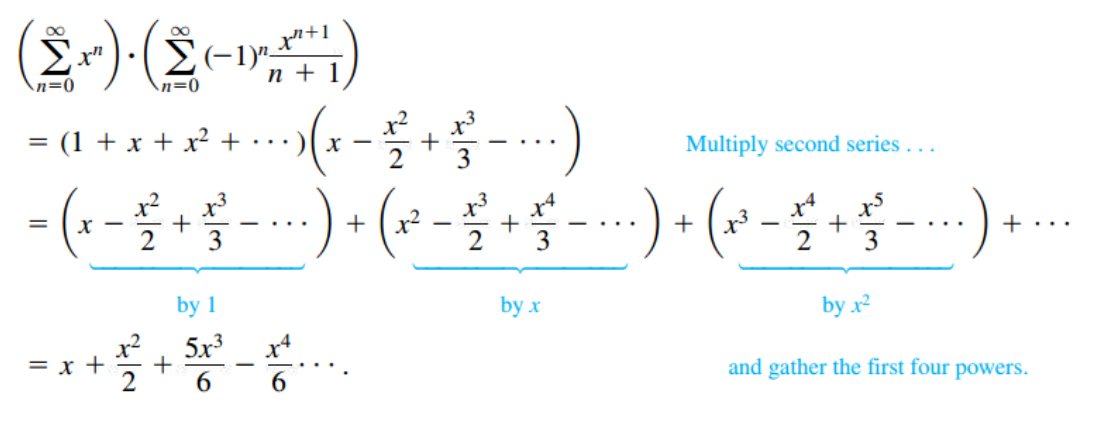
\includegraphics[width = 0.95\textwidth]{./img/thm19ex.png}

\end{center}

\section{Substituting Functions into Convergent Power Series}
Much as we are able to multiply power series within
their overlapping intervals of convergence,
we are also able to substitute functions whose values are
within the interval of convergence $ |f(x)| < R $ into
different power series.

\begin{center}
  \fbox{
    \parbox{\textwidth} {
      \begin{definition}
        Theorem 20 (Subsituting Functions into Power
        Series)
      \end{definition}
      If $ \sum_{n=0}^{\infty} a_{n}x^{n}$ converges
      absolutely for $ |x| < R $ and $ f $ is a continuous
      function, then $ \sum_{n=0}^{\infty} a_{n}(f(x))^{n}$
      converges absolutely on the set of points
      $ x $such that the range of the function $ f(x)$
      is within the radius of convergence, or $ |f(x)| < R $.
    }
  }
\end{center}

\begin{remark*}[(2) Substituting Functions into Power Series]
  Determine the interval of convergence for the following
  power series only using subsitution.
  \[ \sum_{n=0}^{\infty} (4x^{2})^{n}\]
\end{remark*}
Whenever we are approaching this problem, we can observe
what we do know. In the former section, we observed that the
power series
\[ \sum_{n=0}^{\infty} x^{n} \]
will converge for all values of $ |x| < 1 $, since we
are able to think of the power series as a geometric series.
We know that the power series, in this specific case,
will converge to the value
\[ \frac{1}{1-x}\]
Since we know that the function $ 4x^{2}$ is continuous,
then we are able to substitute $ x $ for $ 4x^{2}$, and see
that power series represents the function
\[ \frac{1}{1-4x^{2}}\] and, most importantly,
will converge for the expression $ |x| < 1 \to |4x^{2}| < 1 $.
From evaluating the inequality, we observe that the power series $ \sum_{n=0}^{\infty} (4x^{2})^{n}$
will converge at $ |x| < \frac{1}{2}$.

In addition to being able to add power series, mulitply
power series, and even substitute functions into power series,
we are also able to \textbf{differentiate power series term by term
for all values of $ x $ within their interval of convergence}.

\subsection{Term-By-Term Differentation of Power Series}
\begin{center}
  \fbox{
    \parbox{\textwidth} {
      \begin{definition}
        (Theorem 21) Term-By-Term Differentiation
      \end{definition}
      If $ \sum c_{n}(x-a)^{n} $has the radius of convergence
      $ R > 0 $, it defines a function
      \[ f(x) = \sum_{n=0}^{\infty} c_{n}(x-a)^{n} \textrm{ on the interval }
        a - R < x < a + R \]
      This function $ f $ has derivatives of all orders inside the interval, and we
      obtain the derivatives by differentiating the original series term by term. Here
      are the derivatives of a power series.
      \[ f'(x) = \sum_{n=1}^{\infty} nc_{n}(x-a)^{n-1}\]
      \[ f''(x) = \sum_{n=2}^{\infty} n(n-1)c_{n}(x-a)^{n-2}\]
      and so on. Each of these derived series converges at every point of the
      interval $ a - R < x < a +R $, which is consistent between
      \textit{all derivatives}.
    }
  }
\end{center}
Essentially, we are able to find the \textbf{derivatives} of terms within
a power series that are within the interval of convergence of that power series. We
find the derivatives of the power series (that is, the expression that defines
the power series) by literally finding the derivatives of each term and generating
a new power series expression from it.
\par \textbf{Note:} Whenever we are evaluating the derivative of a
power series, note how we change the \textbf{starting index}.
The reason that this is, is that, whenever we actually derive the power series,
the resulting function will always have an exponent of $ n - a $, such that
a is just some number. This means that at $ n =0 $, the initial term will
always be zero. Therefore, we just reindex the derivative of hte power series
in order to avoid this initial zero.
\par \textbf{Note:} Term-by-term differentation does not work for \textit{all}
power series. For example, if we use the trigonometric series
\[ \sum_{n=0}^{\infty} \frac{sin(n!x)}{n^{2}}  \]
converges for all $ x $. But if we differentaite term by term
we obtain the following series
\[ \sum_{n=1}^{\infty} \frac{n!\cos{n!x}}{n^{2}} \]
which diverges for all $ x $. Note how these two series are \textbf{not}
power series, since they are not a sum of \textit{positive integer powers of $x$ }.
\\ \\
In addition to being able to differentiate a power series, we are also able to
\textit{integrate} a power series and find antiderivatives that exist on
the same interval of convergence.

\subsection{Term-By-Term Integration}
\begin{center}
  \fbox{
    \parbox{\textwidth} {
      \begin{definition}
        (Theorem 22) Term-By-Term Integration

      \end{definition}
      Suppose that
      \[ f(x) = \sum_{n=0}^{\infty} c_{n}(x-a)^{n} \]
      converges for $ a - R < x < a + R (R > 0) $. Then
      \[ \sum_{n=0}^{\infty} c_{n} \frac{(x-a)^{n+1}}{n+1}\]
      converges for $ a - R < x < a + R (R > 0) $ and
      \[ \int_{}^{} f(x)dx =  \sum_{n=0}^{\infty} c_{n} \frac{(x-a)^{n+1}}{n+1} + C \]
      for $ a - R < x < a + R $.
    }
  }
\end{center}
  The consequences of being able to manipualte series like this is that
  we're able to find sequences that have the same exact radius of
  convergence, which allows us to discover functions that
  behave in similar ways (although, of course, not
  in the same exact way). In the given examples, we
  differentiate and integrate power series, starting with
  a power series, then integrating it, only to find it
  to resemble a more familar power series of which
  we know the point of convergence (or the fucntino that
  the power series represents), and then we can just
  integrate that function to find what the original
  power series represents.
  \par It is important to understand that whenever
  we are integrating a power series, we are
  literally integrating all of the terms of
  the power series, similarly to how when
  we differentiate a power series, we are
  literally differentiating all of the terms
  of the power series. We are obtianing
  a series that, although is not going
  to yield the same sum as the original
  function, will behave similarly to the
  original function, albeit with different
  centers, for example. It is important
  for us to be able to freely differentiate
  and integrate series as well as multiply and
  divide them.
  The general form for differentiation and
  integration is as follows
  \[ \frac{d}{dx} \sum_{n=0}^{\infty} c_{n}x^{n} = nc_{n}x^{n-1}\]
  \[ \frac{d^{2}}{dx^{2}} \sum_{n=0}^{\infty} c_{n}x^{n} = (n-1)nc_{n}x^{n-2}\]
  As for integration:
  \[ \int c_{n}(x-a)^{n} dx  = \sum_{n=0}^{\infty} c_{n} \frac{(x-a)^{n+1}}{n+1} + C \]

\chapter{10.7 (Part Four): Manipulation of Series (Part Two)}
\section{Reminders (as of (05/05/23))}
\subsection{MATH\_226}
\begin{enumerate}
  \item  \textbf{Midterm 2} is on \textbf{Tuesday, May 15th, 2023}, which is \textbf{10 days away.}
  \item Remember to revise \textbf{MyLab 15:
        Applications of Taylor Series}.
  \item \textbf{MyLab 16: Complex Numbers} is
        due \textbf{tomorrow, Saturday, May 06, 2023.}
  \item \textbf{Written Homework 7} is due on
        \textbf{Friday, May 12, 2023}.
\end{enumerate}
\subsection{MATH\_230}
\begin{enumerate}
  \item \textbf{230 Midterm 2} is in \textbf{10 days} on
        \textbf{Tuesday, May 15, 2023}.
  \item \textbf{MLM 12: Functions of Multiple Variables} needs revisio n
  \item \textbf{MLM 13: Limits and Continuity in Higher
        Dimensions} is due on \textbf{Sunday, May 7, 2023}.
  \item \textbf{MLM 14: Partial Derivatives} is due on
        \textbf{Tuesday, May 9, 2023.}
        \textbf \textbf{MLM 15: The Chain Rule} is due on
        \textbf{Thursday, May 11, 2023.}
  \item \textbf{WHW 4} is due on \textbf{Wednesday,
        May 10, 2023}.

\end{enumerate}


\section{Objectives}
\begin{enumerate}
  \item Multiply, differentiate, and integrate convergent
        power series
  \item Compose a convergent power series with a
        monomial function to generate new power series
  \item Compute power series rperesentations of several
        elementary functions by manipualting known
        convergent power series
  \item Explain the connection between the coefficients
        of a power series and the sum of a power series
\end{enumerate}

\section{Motivation}
\chapter{10.8 (Part One): Taylor Series}
\section{Reminders (as of (05/05/23))}
\subsection{MATH\_226}
\begin{enumerate}
  \item  \textbf{Midterm 2} is on \textbf{Tuesday, May 15th, 2023}, which is \textbf{10 days away.}
  \item Remember to revise \textbf{MyLab 15:
        Applications of Taylor Series}.
  \item \textbf{MyLab 16: Complex Numbers} is
        due \textbf{tomorrow, Saturday, May 06, 2023.}
  \item \textbf{Written Homework 7} is due on
        \textbf{Friday, May 12, 2023}.
\end{enumerate}
\subsection{MATH\_230}
\begin{enumerate}
  \item \textbf{230 Midterm 2} is in \textbf{10 days} on
        \textbf{Tuesday, May 15, 2023}.
  \item \textbf{MLM 12: Functions of Multiple Variables} needs revisio n
  \item \textbf{MLM 13: Limits and Continuity in Higher
        Dimensions} is due on \textbf{Sunday, May 7, 2023}.
  \item \textbf{MLM 14: Partial Derivatives} is due on
        \textbf{Tuesday, May 9, 2023.}
        \textbf \textbf{MLM 15: The Chain Rule} is due on
        \textbf{Thursday, May 11, 2023.}
  \item \textbf{WHW 4} is due on \textbf{Wednesday,
        May 10, 2023}.

\end{enumerate}

\section{Objectives}
\begin{enumerate}
  \item Compute the Taylor (as well as MacLaurin) seires
        generated by an infinitely differentiable
        fucntion centered at a given point.
  \item Explore the relationships between the
        coefficient sof a power series and the sum of the
        same power series
\end{enumerate}

\section{Motivation}
\chapter{10.8 (Part Two): Taylor Polynomials and
Taylor Series Convergence }
\section{Reminders (as of (05/05/23))}
\subsection{MATH\_226}
\begin{enumerate}
  \item  \textbf{Midterm 2} is on \textbf{Tuesday, May 15th, 2023}, which is \textbf{10 days away.}
  \item Remember to revise \textbf{MyLab 15:
        Applications of Taylor Series}.
  \item \textbf{MyLab 16: Complex Numbers} is
        due \textbf{tomorrow, Saturday, May 06, 2023.}
  \item \textbf{Written Homework 7} is due on
        \textbf{Friday, May 12, 2023}.
\end{enumerate}
\subsection{MATH\_230}
\begin{enumerate}
  \item \textbf{230 Midterm 2} is in \textbf{10 days} on
        \textbf{Tuesday, May 15, 2023}.
  \item \textbf{MLM 12: Functions \section{Reminders (as of (05/05/23))}
\subsection{MATH\_226}
\begin{enumerate}
  \item  \textbf{Midterm 2} is on \textbf{Tuesday, May 15th, 2023}, which is \textbf{10 days away.}
  \item Remember to revise \textbf{MyLab 15:
        Applications of Taylor Series}.
  \item \textbf{MyLab 16: Complex Numbers} is
        due \textbf{tomorrow, Saturday, May 06, 2023.}
  \item \textbf{Written Homework 7} is due on
        \textbf{Friday, May 12, 2023}.
\end{enumerate}
\subsection{MATH\_230}
\begin{enumerate}
  \item \textbf{230 Midterm 2} is in \textbf{10 days} on
        \textbf{Tuesday, May 15, 2023}.
  \item \textbf{MLM 12: Functions of Multiple Variables} needs revisio n
  \item \textbf{MLM 13: Limits and Continuity in Higher
        Dimensions} is due on \textbf{Sunday, May 7, 2023}.
  \item \textbf{MLM 14: Partial Derivatives} is due on
        \textbf{Tuesday, May 9, 2023.}
        \textbf \textbf{MLM 15: The Chain Rule} is due on
        \textbf{Thursday, May 11, 2023.}
  \item \textbf{WHW 4} is due on \textbf{Wednesday,
        May 10, 2023}.

\end{enumerate}

\section{Motivation}of Multiple Variables} needs revisio n
  \item \textbf{MLM 13: Limits and Continuity in Higher
        Dimensions} is due on \textbf{Sunday, May 7, 2023}.
  \item \textbf{MLM 14: Partial Derivatives} is due on
        \textbf{Tuesday, May 9, 2023.}
        \textbf \textbf{MLM 15: The Chain Rule} is due on
        \textbf{Thursday, May 11, 2023.}
  \item \textbf{WHW 4} is due on \textbf{Wednesday,
        May 10, 2023}.

\end{enumerate}

\section{Motivation}
\section{Reminders (as of (05/05/23))}
\subsection{MATH\_226}
\begin{enumerate}
  \item  \textbf{Midterm 2} is on \textbf{Tuesday, May 15th, 2023}, which is \textbf{10 days away.}
  \item Remember to revise \textbf{MyLab 15:
        Applications of Taylor Series}.
  \item \textbf{MyLab 16: Complex Numbers} is
        due \textbf{tomorrow, Saturday, May 06, 2023.}
  \item \textbf{Written Homework 7} is due on
        \textbf{Friday, May 12, 2023}.
\end{enumerate}
\subsection{MATH\_230}
\begin{enumerate}
  \item \textbf{230 Midterm 2} is in \textbf{10 days} on
        \textbf{Tuesday, May 15, 2023}.
  \item \textbf{MLM 12: Functions of Multiple Variables} needs revisio n
  \item \textbf{MLM 13: Limits and Continuity in Higher
        Dimensions} is due on \textbf{Sunday, May 7, 2023}.
  \item \textbf{MLM 14: Partial Derivatives} is due on
        \textbf{Tuesday, May 9, 2023.}
        \textbf \textbf{MLM 15: The Chain Rule} is due on
        \textbf{Thursday, May 11, 2023.}
  \item \textbf{WHW 4} is due on \textbf{Wednesday,
        May 10, 2023}.

\end{enumerate}

\section{Motivation}

\chapter{Convergence of Taylor Series ((05/05/23))}
\section{Reminders (as of (05/05/23))}
\subsection{MATH\_226}
\begin{enumerate}
  \item  \textbf{Midterm 2} is on \textbf{Tuesday, May 15th, 2023}, which is \textbf{10 days away.}
  \item Remember to revise \textbf{MyLab 15:
        Applications of Taylor Series}.
  \item \textbf{MyLab 16: Complex Numbers} is
        due \textbf{tomorrow, Saturday, May 06, 2023.}
  \item \textbf{Written Homework 7} is due on
        \textbf{Friday, May 12, 2023}.
\end{enumerate}
\subsection{MATH\_230}
\begin{enumerate}
  \item \textbf{230 Midterm 2} is in \textbf{10 days} on
        \textbf{Tuesday, May 15, 2023}.
  \item \textbf{MLM 12: Functions of Multiple Variables} needs revisio n
  \item \textbf{MLM 13: Limits and Continuity in Higher
        Dimensions} is due on \textbf{Sunday, May 7, 2023}.
  \item \textbf{MLM 14: Partial Derivatives} is due on
        \textbf{Tuesday, May 9, 2023.}
        \textbf \textbf{MLM 15: The Chain Rule} is due on
        \textbf{Thursday, May 11, 2023.}
  \item \textbf{WHW 4} is due on \textbf{Wednesday,
        May 10, 2023}.

\end{enumerate}

\section{Motivation}

\chapter{Applications of Taylor Series}
\section{Reminders (as of (05/05/23))}
\subsection{MATH\_226}
\begin{enumerate}
  \item  \textbf{Midterm 2} is on \textbf{Tuesday, May 15th, 2023}, which is \textbf{10 days away.}
  \item Remember to revise \textbf{MyLab 15:
        Applications of Taylor Series}.
  \item \textbf{MyLab 16: Complex Numbers} is
        due \textbf{tomorrow, Saturday, May 06, 2023.}
  \item \textbf{Written Homework 7} is due on
        \textbf{Friday, May 12, 2023}.
\end{enumerate}
\subsection{MATH\_230}
\begin{enumerate}
  \item \textbf{230 Midterm 2} is in \textbf{10 days} on
        \textbf{Tuesday, May 15, 2023}.
  \item \textbf{MLM 12: Functions of Multiple Variables} needs revisio n
  \item \textbf{MLM 13: Limits and Continuity in Higher
        Dimensions} is due on \textbf{Sunday, May 7, 2023}.
  \item \textbf{MLM \section{Reminders (as of (05/05/23))}
\subsection{MATH\_226}
\begin{enumerate}
  \item  \textbf{Midterm 2} is on \textbf{Tuesday, May 15th, 2023}, which is \textbf{10 days away.}
  \item Remember to revise \textbf{MyLab 15:
        Applications of Taylor Series}.
  \item \textbf{MyLab 16: Complex Numbers} is
        due \textbf{tomorrow, Saturday, May 06, 2023.}
  \item \textbf{Written Homework 7} is due on
        \textbf{Friday, May 12, 2023}.
\end{enumerate}
\subsection{MATH\_230}
\begin{enumerate}
  \item \textbf{230 Midterm 2} is in \textbf{10 days} on
        \textbf{Tuesday, May 15, 2023}.
  \item \textbf{MLM 12: Functions of Multiple Variables} needs revisio n
  \item \textbf{MLM 13: Limits and Continuity in Higher
        Dimensions} is due on \textbf{Sunday, May 7, 2023}.
  \item \textbf{MLM 14: Partial Derivatives} is due on
        \textbf{Tuesday, May 9, 2023.}
        \textbf \textbf{MLM 15: The Chain Rule} is due on
        \textbf{Thursday, May 11, 2023.}
  \item \textbf{WHW 4} is due on \textbf{Wednesday,
        May 10, 2023}.

\end{enumerate}

\section{Motivation}14: Partial Derivatives} is due on
        \textbf{Tuesday, May 9, 2023.}
        \textbf \textbf{MLM 15: The Chain Rule} is due on
        \textbf{Thursday, May 11, 2023.}
  \item \textbf{WHW 4} is due on \textbf{Wednesday,
        May 10, 2023}.

\end{enumerate}

\section{Objectives}
\begin{enumerate}
  \item Explore advanced application sof Taylor
        Series representations to major topics in
        single-variable calculus
\end{enumerate}

\section{Motivation}
\chapter{A7 (Part One): Complex Numbers (Part One)}
\section{Reminders (as of (05/05/23))}
\subsection{MATH\_226}
\begin{enumerate}
  \item  \textbf{Midterm 2} is on \textbf{Tuesday, May 15th, 2023}, which is \textbf{10 days away.}
  \item Remember to revise \textbf{MyLab 15:
        Applications of Taylor Series}.
  \item \textbf{MyLab 16: Complex Numbers} is
        due \textbf{tomorrow, Saturday, May 06, 2023.}
  \item \textbf{Written Homework 7} is due on
        \textbf{Friday, May 12, 2023}.
\end{enumerate}
\subsection{MATH\_230}
\begin{enumerate}
  \item \textbf{230 Midterm 2} is in \textbf{10 days} on
        \textbf{Tuesday, May 15, 2023}.
  \item \textbf{MLM 12: Functions of Multiple Variables} needs revisio n
  \item \textbf{MLM 13: Limits and Continuity in Higher
        Dimensions} is due on \textbf{Sunday, May 7, 2023}.
  \item \textbf{MLM 14: Partial Derivatives} is due on
        \textbf{Tuesday, May 9, 2023.}
        \textbf \textbf{MLM 15: The Chain Rule} is due on
        \textbf{Thursday, May 11, 2023.}
  \item \textbf{WHW 4} is due on \textbf{Wednesday,
        May 10, 2023}.

\end{enumerate}

\section{Objectives}
\begin{enumerate}
  \item Explain the significance of the complex number
        systems via the \textbf{Fundamental Theorem of
        Calcuslu}.
  \item Compute the complex conjugate and absolute
        value of a ocmplex number
  \item Algebraically manipulate algebraic expressions
        involving complex numbers
\end{enumerate}

\section{Motivation}
\chapter{10.10, A7 (Part Two): Complex Numbers (Part Two)}
\section{Reminders (as of (05/05/23))}
\subsection{MATH\_226}
\begin{enumerate}
  \item  \textbf{Midterm 2} is on \textbf{Tuesday, May 15th, 2023}, which is \textbf{10 days away.}
  \item Remember to revise \textbf{MyLab 15:
        Applications of Taylor Series}.
  \item \textbf{MyLab 16: Complex Numbers} is
        due \textbf{tomorrow, Saturday, May 06, 2023.}
  \item \textbf{Written Homework 7} is due on
        \textbf{Friday, May 12, 2023}.
\end{enumerate}
\subsection{MATH\_230}
\begin{enumerate}
  \item \textbf{230 Midterm 2} is in \textbf{10 days} on
        \textbf{Tuesday, May 15, 2023}.
  \item \textbf{MLM 12: Functions of Multiple Variables} needs revisio n
  \item \textbf{MLM 13: Limits and Continuity in Higher
        Dimensions} is due on \textbf{Sunday, May 7, 2023}.aaaa
  \item \textbf{MLM 14: Partial Derivatives} is due on
        \textbf{Tuesday, May 9, 2023.}
        \textbf \textbf{MLM 15: The Chain Rule} is due on
        \textbf{Thursday, May 11, 2023.}
  \item \textbf{WHW 4} is due on \textbf{Wednesday,
        May 10, 2023}.

\end{enumerate}

\section{Objectives}
\begin{enumerate}
  \item Understand Euler's fomrula and the polar coordinate
        representations of complex numbers
  \item Be able to visualize the ocmplex plane as
        well as points and expressions of the ocmplex plane
  \item Be able to manipulate the exponential function
        and investigate its propertie sin reltaion to
        complex numbers
        \item Establish roots of unity and \textbf{DeMoivre numbers and theoerems}.

\end{enumerate}

\section{Motivation}
\chapter{19.1 (Part One): Vectors}
\section{Reminders}
\section{Motivation}
\chapter{19.1 (Part Two): Inner Products}
\section{Reminders}
\section{Motivation}
